\appendixsection{Детали эксперимента}

\subsection*{Параметры устройства}

Эксперимент проводился на сверхпроводящем квантовом процессоре
flip‑chip‑типа \cite{cite_44} с 10 кубитами (Q1–Q10) и 9 соединителями (C1–C9),
попеременно расположенными в цепочечной топологии (рис. \ref{fig:fig02}A). Все
кубиты и соединители — трансмоны; их частоты настраиваются независимо при
помощи медленных потоковых импульсов (длительностью до сотен микросекунд) либо
быстрых Z‑импульсов (до десятков микросекунд) по соответствующим управляющим
линиям. Максимальные частоты кубитов (соединителей) $\approx$ 4.7 ГГц (9.0
ГГц), нелинейности $\approx$ -210 МГц (-150 МГц). Силе связи соседних кубитов
регулируется от почти нуля до -10 МГц модуляцией частоты промежуточного
соединителя. По управляющим линиям кубитов также подаются СВЧ‑импульсы для
однокубитных затворов. Времена релаксации, дефазировки, достоверности затворов
и иные характеристики сведены в табл. Д.8.

\begin{table}[h]
    \centering
    \caption{
        Параметры устройства. $\omega^{0}_{j}$ — это частота покоя кубита
        $Q_{j}$ (idle frequency), при которой кубит инициализируется.
        $\eta_{j}$ — это нелинейность кубита $Q_{j}$. $T_{1,j}$ и $T_{2,j}$ —
        соответственно время релаксации энергии и время дефазировки Рамсе
        кубита $Q_{j}$ на частоте покоя. $F_{0,j}$ и $F_{1,j}$ — фиделити
        измерения кубита $Q_{j}$, подготовленного в состояниях $\lvert
        0\rangle$ и $\lvert 1\rangle$ соответственно. $e^{S}_{j}$ —
        одновременная ошибка Паули однокубитного затвора кубита $Q_{j}$.
        $e^{\text{CZ}}_{j,A(B)}$ — одновременная ошибка Паули CZ‑затвора
        кубитов $Q_{j}$ и $Q_{j+1}$ в группе~A (B).
        $(\omega^{A(B)}_{j},\,\omega^{A(B)}_{j+1})$ — оценочные частоты кубитов
        $Q_{j}$ и $Q_{j+1}$ в группе~A (B) при выполнении CZ‑затворов. }

    \resizebox{\textwidth}{!}{%
        \begin{tabular}{c|c|c|c|c|c|c|c|c|c|c|c}
        \hline\hline
            Кубит & Q$_1$ & Q$_2$ & Q$_3$ & Q$_4$ & Q$_5$ & Q$_6$ & Q$_7$ & Q$_8$ & Q$_9$ & Q$_{10}$ & среднее \\
            \hline
            $\omega_j^0/2\pi$ (GHz) & 4.420 & 4.200 & 4.553 & 4.460 & 4.370 & 4.600 & 4.430 & 4.515 & 4.445 & 4.570 & 4.486 \\
            \hline
            $\eta_j/2\pi$ (MHz) & -213 & -209 & -208 & 209 & -211 & -211 & -209 & -210 & -211 & -210 & -210 \\
            \hline
            $T_{1,j}$ ($\mu$s) & 91.4 & 83.3 & 113.6 & 131.1 & 111.6 & 99.5 & 116.0 & 108.2 & 123.3 & 115.1 & 109.3 \\
            \hline
            $T_{2,j}$ ($\mu$s) & 5.3 & 7.0 & 5.7 & 4.3 & 6.2 & 4.9 & 5.8 & 8.2 & 6.9 & 5.9 & 6.2 \\
            \hline
            $F_{0,j}$ ($\mu$s) & 0.982 & 0.984 & 0.996 & 0.991 & 0.992 & 0.990 & 0.981 & 0.978 & 0.974 & 0.978 & 0.981 \\
            \hline
            $F_{1,j}$ ($\mu$s) & 0.949 & 0.967 & 0.942 & 0.957 & 0.951 & 0.958 & 0.960 & 0.958 & 0.927 & 0.923 & 0.949 \\
            \hline
            $\epsilon_j^S$ (\%) & 0.11 & 0.07 & 0.09 & 0.09 & 0.15 & 0.12 & 0.07 & 0.08 & 0.09 & 0.09 & 0.09 \\
            \hline
            \end{tabular}
    }

\resizebox{\textwidth}{!}{%
\begin{tabular}{c|c|c|c|c|c|c}
\hline
Кубит & Q$_1$-Q$_2$ & Q$_3$-Q$_4$ & Q$_5$-Q$_6$ & Q$_7$-Q$_8$ & Q$_9$-Q$_{10}$ & среднее \\
\hline
$(\omega_j^A, \omega_{j+1}^A)/2\pi$ (GHz) & 4.315, 4.520 & 4.666, 4.460 & 4.600, 4.392 & 4.335, 4.540 & 4.570, 4.364 & - \\
\hline
$\epsilon_{j,A}^{CZ}$ (\%) & 0.65 & 0.72 & 0.65 & 0.67 & 0.76 & 0.69 \\
\hline
\end{tabular}
}

\resizebox{\textwidth}{!}{%
\begin{tabular}{c|c|c|c|c|c|c|c}
\hline
Кубит & Q$_1$ & Q$_2$-Q$_3$ & Q$_4$-Q$_5$ &Q$_6$-Q$_7$ &Q$_8$-Q$_9$ & Q$_{10}$ & среднее \\
\hline
$(\omega_j^B, \omega_{j+1}^B)/2\pi$ (GHz) & - & 4.348, 4.553 & 4.510, 4.304 & 4.609, 4.400 & 4.532, 4.325 & - & - \\
\hline
$\epsilon_{j,B}^{CZ}$ (\%) & - & 0.54 & 0.70 & 0.58 & 0.57 & - & 0.60 \\
\hline
\hline
\end{tabular}
}
    \label{tab:tab10}
\end{table}


\subsection*{Калибровка экспериментальных затворов}

Все кубиты инициализируются в основное состояние процедурой сброса:
соединитель, соседний кубиту, резонансно сводится с ним на несколько
наносекунд, что переносит возбуждение в соединитель; далее соединитель
переводится на максимальную частоту, где его $T_{1}$ мало, и возбуждение быстро
распадается. Шаги повторяются до полной инициализации. Затем реализуются
экспериментальные схемы (рис. \ref{fig:fig02}D). Для длинных пауз вставляются
двойные $R_{x}(\pi)$‑затворы, чтобы защитить кубит от дефазировки. После
измерения сырых вероятностей строк битов проводится коррекция чтения
\cite{cite_45}.

Экспериментальная схема содержит затворы $R_{x}(\theta),R_{y}(\theta),R_{z}
(\theta)$ (вращения на $x,y,z$ на угол $\theta$), Адамара и затворы
с контролируемой фазой (CZ). $R_{x}$, $R_{y}$ реализуются 30‑нс СВЧ‑импульсами
с заданными фазами и амплитудами. $R_{z}$ реализуются виртуальными Z затворами,
которые могут считаться идеальными затворами, которые занимают нулевое
время путем изменением фаз последующих импульсов \cite{cite_46}. Затвор Адамара
реализуется как $H = R_{y}(\pi/2)R_{z}(\pi)$. CZ‑затворы выполняются специально
сформированными потоковыми импульсами, воздействующими на соседние кубиты
и общий соединитель; детали описаны в \cite{cite_34,cite_47}. По возможности
последовательные однокубитные затворы объединяются, уменьшая глубину схемы.

Здесь мы обсуждаем случай оптимизации фиделити затворов при выполнении
CZ‑затворов параллельно, что аналогично индивидуальной реализации, за
исключением оптимизации параметров импульсов для соединителей. В соответствии с
требованиями экспериментальной схемы, мы делим девять соединителей на две
группы: $\{C_1, C_3, C_5, C_7, C_9\}$ для группы~A и $\{C_2, C_4, C_6, C_8\}$
для группы~B.  Мы одновременно применяем прямоугольные магнитные импульсы с
синусоидальной модуляцией вида $A(t) = z_{C_j} \cdot \left( 1 - r_{C_j} +
r_{C_j} \sin\left( \frac{\pi t}{t_{\text{gate}}} \right) \right)$ ко всем
соединителям в группе~A или~B. Здесь $z_{C_j}$ — это максимальная амплитуда
потока, приложенного к соединителю $C_j$, $r_{C_j}$ — модульный параметр,
зафиксированный около 0{,}1, а $t_{\text{gate}} = 50$~нс. Обрати внимание, что
5-нс интервалы добавляются до и после этого магнитного импульса. Для
оптимизации $z_{C_j}$ мы подготавливаем кубиты $Q_j$ и $Q_{j+1}$ в состоянии
$\lvert 11 \rangle$ и применяем $m$ циклов CZ‑затворов при $m \in \{1, 3, 5\}$.
Затем мы напрямую измеряем утечку в состояние $\lvert 2 \rangle$ у кубита с
более высокой резонансной частотой в паре, и минимизируем эту утечку для всех
пар одновременно путём тонкой настройки всех $z_{C_i}$.

Мы используем кросс-энтропийный бенчмаркинг (XEB)~\cite{cite_2} для оценки
производительности наших квантовых затворов. Средняя ошибка Паули для
одновременных однокубитных затворов составляет 0{,}09\%. Средние ошибки Паули
для CZ‑затворов в группах~A и~B составляют 0{,}69\% и 0{,}60\% соответственно.
Следует отметить, что структура экспериментальной схемы отличается от
стандартных схем оценки производительности. В связи с этим мы используем
альтернативные квантовые схемы для дополнительной верификации
производительности наших CZ‑затворов, которые имеют структуры, схожие со
схемами, используемыми в нашем алгоритме (см. рис. \ref{fig:fig05}). На рис.
\ref{fig:fig05}C показана точность XEB в зависимости от глубины схемы
(количества циклов), демонстрируя ошибку цикла порядка 3{,}45\%, на основе чего
мы оцениваем среднюю ошибку CZ‑затвора как 0{,}55\%.

\begin{figure}
    \centering
    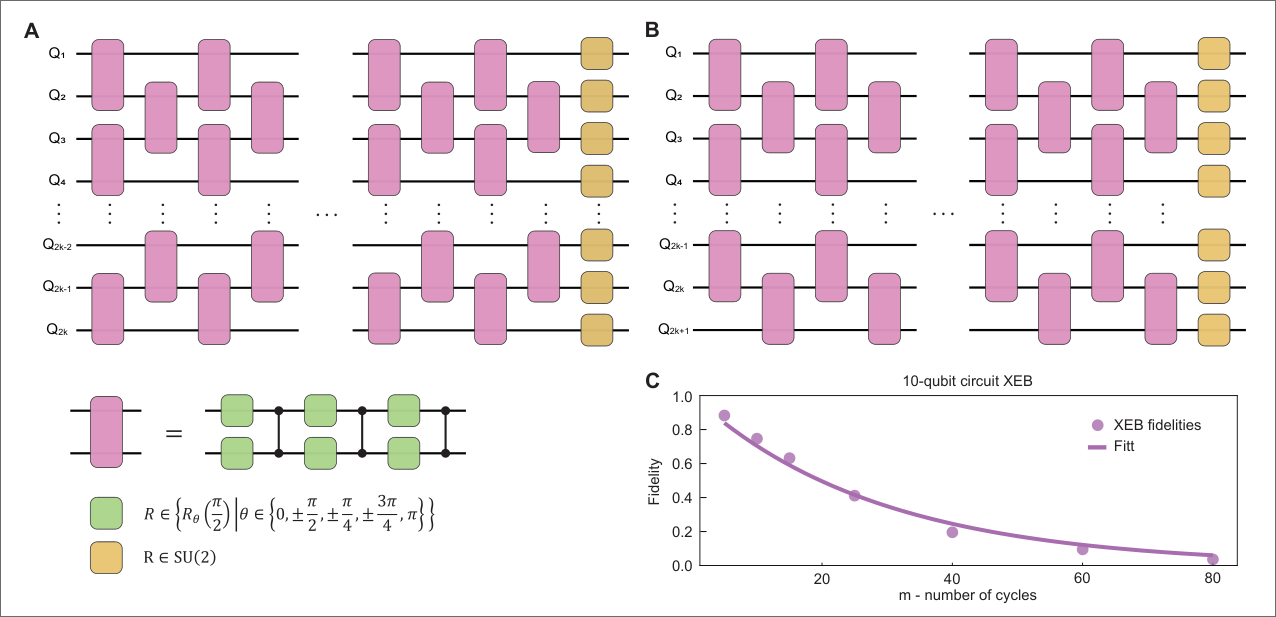
\includegraphics[scale=0.35]{inc/fig_05.png}
    \caption{
    Альтернативные квантовые схемы, используемые для бенчмаркинга CZ‑затворов,
    для чётного (A) и нечётного (B) числа кубитов. Зелёные квадраты обозначают
    случайно выбранные полу‑$\pi$‑повороты вокруг восьми осей, где $\theta$ —
    угол между осью поворота и осью $x$. Жёлтые квадраты обозначают затворы,
    случайно выбранные из $\mathrm{SU}(2)$. C, фиделити XEB как функция числа
    циклов затвора для случая с 10 кубитами. Ошибка цикла аппроксимирована
    значением около 3{,}45\,\%, причём каждый цикл содержит слой из 11
    однокубитных затворов, за которым в среднем следует слой из 4{,}5
    CZ‑затворов.
    }
    \label{fig:fig05}
\end{figure}

\subsection*{Процедура QAOA и сходимость}

QAOA может находить приближённое основное состояние гамильтониана путём
обновления параметров. Для QAOA с $p$ слоями участвуют $2p$ вариационных
параметров: $\boldsymbol{\gamma} = (\gamma_1, ..., \gamma_p)$ и
$\boldsymbol{\beta} = (\beta_1, ..., \beta_p)$. Основная задача квантового
процессора — многократно подготавливать следующую параметрическую волновую
функцию:

\begin{equation}
\lvert \gamma, \beta \rangle
      = e^{-i\beta_{p} H_{b}}
        e^{-i\gamma_{p} H_{c}}
        \dots
        e^{-i\beta_{1} H_{b}}
        e^{-i\gamma_{1} H_{c}}
        \lvert + \rangle^{n},
\end{equation}

\noindent где $H_b = \sum_{j=1}^{n} \sigma_x^j$ — это смешивающий гамильтониан. Это
состояние может быть подготовлено путём чередующегося применения унитарных
операторов $U(H_c, \gamma) = e^{-i\gamma H_c}$ и $U(H_b, \beta) = e^{-i\beta
H_b}$ с разными параметрами к состоянию равномерной суперпозиции $\lvert +
\rangle^{n}$. Классический оптимизатор используется для поиска оптимальных
параметров $(\boldsymbol{\gamma}^*, \boldsymbol{\beta}^*)$, минимизирующих
ожидаемое значение энергии проблемного гамильтониана:

\begin{equation}
E(\gamma, \beta)
      = \langle \gamma, \beta \lvert H_{c} \rvert \gamma, \beta \rangle
\end{equation}

Эта функция энергии может быть вычислена путём многократной подготовки волновой
функции $\lvert \boldsymbol{\gamma}, \boldsymbol{\beta} \rangle$ в квантовом
регистре и её измерения в вычислительном базисе. В результате получается
квантовое состояние $\lvert \boldsymbol{\gamma}^*, \boldsymbol{\beta}^*
\rangle$, соответствующее приближённому решению. Алгоритм графически
представлен на рис. \ref{fig:fig02}C.

Здесь мы кратко представим классический оптимизатор, используемый в QAOA во
время процедуры оптимизации параметров. Оптимизатор называется методом
модельного градиентного спуска (model gradient descent, MGD)~\cite{cite_48}. На
самом деле, можно рассмотреть и множество других классических алгоритмов
оптимизации, таких как метод симплекса Нелдера–Мида~\cite{cite_49},
квазиньютоновские методы~\cite{cite_50,cite_51}. Производительность этих
методов часто зависит от конкретной задачи. Показано как численно, так и
экспериментально, что модельный градиентный спуск работает хорошо для некоторых
вариационных квантовых анзацев~\cite{cite_11,cite_48}. Ключевая идея MGD —
использование модели для оценки градиента целевой функции, которая представляет
собой непрерывную поверхность или гиперповерхность. Для оценки градиента в
данной точке на поверхности случайным образом выбираются несколько близлежащих
точек и вычисляются значения целевой функции в этих точках. Затем квадратичная
модель аппроксимирует поверхность этих точек с помощью метода наименьших
квадратов. Градиент этой квадратичной модели используется в качестве замены
истинного градиента, и алгоритм спускается по соответствующему направлению.
Псевдокод приведён в алгоритме 3.

В нашем эксперименте метод MGD хорошо показал себя в трёх задачах факторизации.
Он сходится к локальному или глобальному оптимуму в пределах 10 шагов из
случайно выбранных начальных точек. При этом экспериментальные результаты
сходимости сопоставимы с теоретическими на текущем масштабе. Подробности о
траекториях сходимости приведены на рис. \ref{fig:fig06}.

\begin{figure}
    \centering
    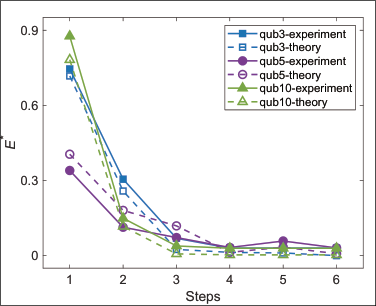
\includegraphics[scale=0.9]{inc/fig_06.png}
    \caption{
    Подробности о траекториях сходимости для трёх задач факторизации. Квадраты,
    кружки и треугольники соответствуют случаям с 3, 5 и 10 кубитами
    соответственно. Сплошные (пустые) символы обозначают экспериментальные
    (теоретические) результаты. По вертикальной оси отложено нормализованное
    значение энергетической функции $E^{*}$, а по горизонтальной оси — шаги
    вычислительной итерации.
    }
    \label{fig:fig06}
\end{figure}

\begin{algorithm}[htp!]
    \SetAlgoLined

    \KwData{начальная точка $x_0$, скорость обучения $\gamma$, радиус выборки $\delta$, количество точек $k$, показатель убывания скорости $\alpha$, постоянная устойчивости $A$, показатель убывания радиуса $\xi$, точность $\varepsilon$, максимальное число итераций $n$}
    \KwResult{оптимальное значение $x$}

    Инициализировать список $L$; \\
    $x \gets x_0$; \\
    $m \gets 0$; \\

    \While{число вычислений функции $+$ $k$ не превышает $n$}{
        Добавить кортеж $(x, f(x))$ в список $L$; \\
        $\delta' \gets \delta / (m + 1)^{\xi}$; \\
        Сэмплировать $k$ точек равномерно случайно из $\delta'$-окрестности $x$; пусть $S$ — полученное множество; \\
        \ForEach{$x' \in S$}{
            Добавить $(x', f(x'))$ в $L$;
        }

        Инициализировать список $L'$; \\
        \ForEach{кортеж $(x', y') \in L$}{
            \If{$\|x' - x\| < \delta'$}{
                Добавить $(x', y')$ в $L'$;
            }
        }

        Аппроксимировать квадратичную модель по точкам из $L'$ с помощью линейной регрессии с полиномиальными признаками; \\
        Пусть $g$ — градиент квадратичной модели в $x$; \\
        $\gamma' \gets \gamma / (m + 1 + A)^{\alpha}$; \\
        \If{$\gamma' \cdot \|g\| < \varepsilon$}{
            \Return $x$;
        }

        $x \gets x - \gamma' \cdot g$; \\
        $m \gets m + 1$;
    }

    \Return $x$;

    \caption{Алгоритм Model Gradient Descent}
    \label{alg:mgd}
\end{algorithm}

